% Created by tikzDevice version 0.7.0 on 2014-01-30 09:59:27
% !TEX encoding = UTF-8 Unicode
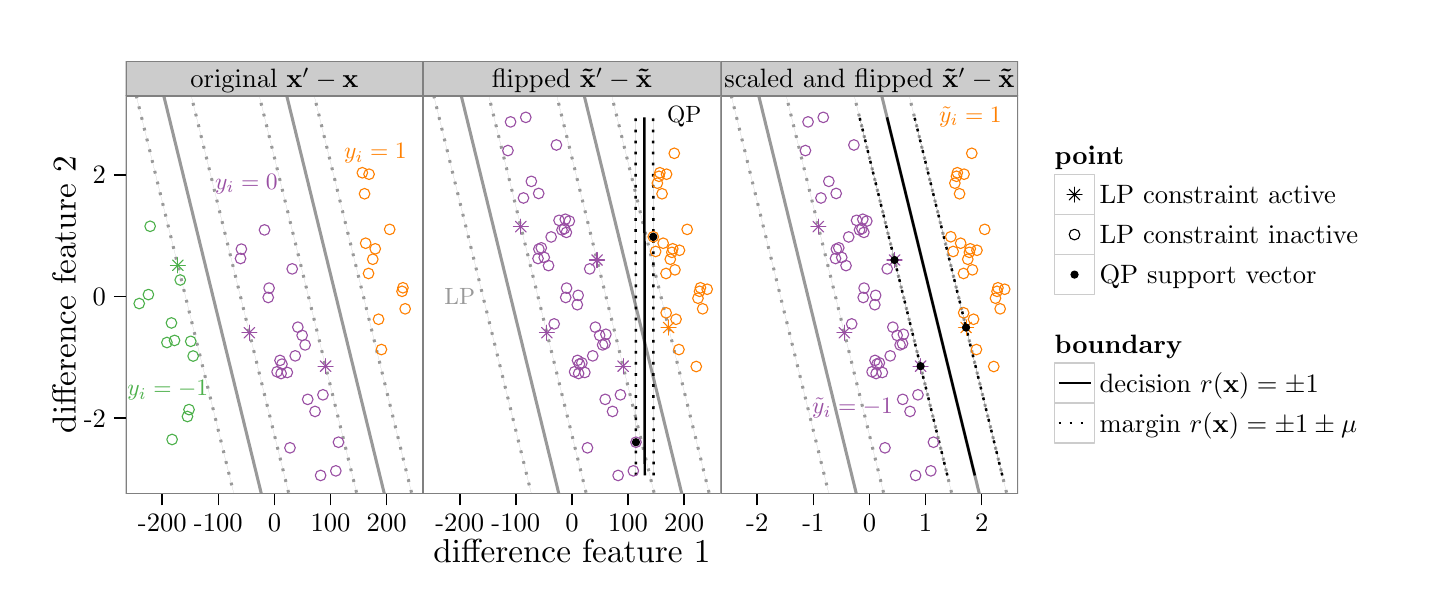
\begin{tikzpicture}[x=1pt,y=1pt]
\definecolor[named]{fillColor}{rgb}{1.00,1.00,1.00}
\path[use as bounding box,fill=fillColor,fill opacity=0.00] (0,0) rectangle (505.89,202.36);
\begin{scope}
\path[clip] (  0.00,  0.00) rectangle (505.89,202.36);
\definecolor[named]{drawColor}{rgb}{1.00,1.00,1.00}
\definecolor[named]{fillColor}{rgb}{1.00,1.00,1.00}

\path[draw=drawColor,line width= 0.6pt,line join=round,line cap=round,fill=fillColor] (  0.00,  0.00) rectangle (505.89,202.36);
\end{scope}
\begin{scope}
\path[clip] ( 35.42,177.68) rectangle (142.92,190.31);
\definecolor[named]{drawColor}{rgb}{0.50,0.50,0.50}
\definecolor[named]{fillColor}{rgb}{0.80,0.80,0.80}

\path[draw=drawColor,line width= 0.6pt,line join=round,line cap=round,fill=fillColor] ( 35.42,177.68) rectangle (142.92,190.31);
\definecolor[named]{drawColor}{rgb}{0.00,0.00,0.00}

\node[text=drawColor,anchor=base,inner sep=0pt, outer sep=0pt, scale=  0.96] at ( 89.17,180.69) {original $\mathbf x'-\mathbf x$};
\end{scope}
\begin{scope}
\path[clip] (142.92,177.68) rectangle (250.42,190.31);
\definecolor[named]{drawColor}{rgb}{0.50,0.50,0.50}
\definecolor[named]{fillColor}{rgb}{0.80,0.80,0.80}

\path[draw=drawColor,line width= 0.6pt,line join=round,line cap=round,fill=fillColor] (142.92,177.68) rectangle (250.42,190.31);
\definecolor[named]{drawColor}{rgb}{0.00,0.00,0.00}

\node[text=drawColor,anchor=base,inner sep=0pt, outer sep=0pt, scale=  0.96] at (196.67,180.69) {flipped $\mathbf{\tilde x'}-\mathbf{\tilde x}$};
\end{scope}
\begin{scope}
\path[clip] (250.42,177.68) rectangle (357.92,190.31);
\definecolor[named]{drawColor}{rgb}{0.50,0.50,0.50}
\definecolor[named]{fillColor}{rgb}{0.80,0.80,0.80}

\path[draw=drawColor,line width= 0.6pt,line join=round,line cap=round,fill=fillColor] (250.42,177.68) rectangle (357.92,190.31);
\definecolor[named]{drawColor}{rgb}{0.00,0.00,0.00}

\node[text=drawColor,anchor=base,inner sep=0pt, outer sep=0pt, scale=  0.96] at (304.17,180.69) {scaled and flipped $\mathbf{\tilde x'}-\mathbf{\tilde x}$};
\end{scope}
\begin{scope}
\path[clip] ( 35.42, 34.03) rectangle (142.92,177.68);
\definecolor[named]{fillColor}{rgb}{1.00,1.00,1.00}

\path[fill=fillColor] ( 35.42, 34.03) rectangle (142.92,177.68);
\definecolor[named]{drawColor}{rgb}{0.60,0.60,0.60}
\definecolor[named]{fillColor}{rgb}{0.60,0.60,0.60}

\path[draw=drawColor,line width= 1.1pt,line join=round,fill=fillColor] ( 43.14,202.36) -- ( 92.76,  0.00);

\path[draw=drawColor,line width= 1.1pt,line join=round,fill=fillColor] ( 87.58,202.36) -- (137.20,  0.00);

\path[draw=drawColor,line width= 1.1pt,dash pattern=on 1pt off 3pt ,line join=round,fill=fillColor] ( 77.65,202.36) -- (127.27,  0.00);

\path[draw=drawColor,line width= 1.1pt,dash pattern=on 1pt off 3pt ,line join=round,fill=fillColor] ( 97.51,202.36) -- (142.92, 17.16);

\path[draw=drawColor,line width= 1.1pt,dash pattern=on 1pt off 3pt ,line join=round,fill=fillColor] ( 35.42,193.35) -- ( 82.83,  0.00);

\path[draw=drawColor,line width= 1.1pt,dash pattern=on 1pt off 3pt ,line join=round,fill=fillColor] ( 53.07,202.36) -- (102.69,  0.00);
\definecolor[named]{drawColor}{rgb}{0.60,0.31,0.64}

\path[draw=drawColor,line width= 0.4pt,line join=round,line cap=round] ( 93.83, 77.77) circle (  1.92);

\path[draw=drawColor,line width= 0.4pt,line join=round,line cap=round] (103.84, 63.69) circle (  1.92);

\path[draw=drawColor,line width= 0.4pt,line join=round,line cap=round] (105.85, 40.56) circle (  1.92);

\path[draw=drawColor,line width= 0.4pt,line join=round,line cap=round] (112.30, 52.56) circle (  1.92);

\path[draw=drawColor,line width= 0.4pt,line join=round,line cap=round] ( 91.58, 77.39) circle (  1.92);

\path[draw=drawColor,line width= 0.4pt,line join=round,line cap=round] (111.35, 42.21) circle (  1.92);

\path[draw=drawColor,line width= 0.4pt,line join=round,line cap=round] (100.25, 87.72) circle (  1.92);

\path[draw=drawColor,line width= 0.4pt,line join=round,line cap=round] ( 91.89, 80.78) circle (  1.92);

\path[draw=drawColor,line width= 0.4pt,line join=round,line cap=round] ( 94.78, 50.54) circle (  1.92);
\definecolor[named]{drawColor}{rgb}{1.00,0.50,0.00}

\path[draw=drawColor,line width= 0.4pt,line join=round,line cap=round] (121.73,142.34) circle (  1.92);

\path[draw=drawColor,line width= 0.4pt,line join=round,line cap=round] (123.36,149.41) circle (  1.92);
\definecolor[named]{drawColor}{rgb}{0.30,0.69,0.29}

\path[draw=drawColor,line width= 0.4pt,line join=round,line cap=round] ( 58.30, 64.35) circle (  1.92);

\path[draw=drawColor,line width= 0.4pt,line join=round,line cap=round] ( 58.92, 89.02) circle (  1.92);

\path[draw=drawColor,line width= 0.4pt,line join=round,line cap=round] ( 57.73, 61.85) circle (  1.92);
\definecolor[named]{drawColor}{rgb}{1.00,0.50,0.00}

\path[draw=drawColor,line width= 0.4pt,line join=round,line cap=round] (120.93,149.94) circle (  1.92);

\path[draw=drawColor,line width= 0.4pt,line join=round,line cap=round] (123.17,113.54) circle (  1.92);
\definecolor[named]{drawColor}{rgb}{0.30,0.69,0.29}

\path[draw=drawColor,line width= 0.4pt,line join=round,line cap=round] ( 59.79, 83.71) circle (  1.92);

\path[draw=drawColor,line width= 0.4pt,line join=round,line cap=round] ( 52.19, 53.55) circle (  1.92);
\definecolor[named]{drawColor}{rgb}{1.00,0.50,0.00}

\path[draw=drawColor,line width= 0.4pt,line join=round,line cap=round] (122.13,124.47) circle (  1.92);
\definecolor[named]{drawColor}{rgb}{0.60,0.31,0.64}

\path[draw=drawColor,line width= 0.4pt,line join=round,line cap=round] ( 99.18, 91.17) circle (  1.92);

\path[draw=drawColor,line width= 0.4pt,line join=round,line cap=round] (101.19, 68.05) circle (  1.92);

\path[draw=drawColor,line width= 0.4pt,line join=round,line cap=round] (105.72, 78.12) -- (109.56, 81.96);

\path[draw=drawColor,line width= 0.4pt,line join=round,line cap=round] (105.72, 81.96) -- (109.56, 78.12);

\path[draw=drawColor,line width= 0.4pt,line join=round,line cap=round] (104.92, 80.04) -- (110.36, 80.04);

\path[draw=drawColor,line width= 0.4pt,line join=round,line cap=round] (107.64, 77.33) -- (107.64, 82.76);

\path[draw=drawColor,line width= 0.4pt,line join=round,line cap=round] ( 86.92,104.87) circle (  1.92);

\path[draw=drawColor,line width= 0.4pt,line join=round,line cap=round] (106.69, 69.69) circle (  1.92);

\path[draw=drawColor,line width= 0.4pt,line join=round,line cap=round] ( 95.59,115.20) circle (  1.92);

\path[draw=drawColor,line width= 0.4pt,line join=round,line cap=round] ( 87.23,108.26) circle (  1.92);

\path[draw=drawColor,line width= 0.4pt,line join=round,line cap=round] ( 90.12, 78.03) circle (  1.92);
\definecolor[named]{drawColor}{rgb}{0.30,0.69,0.29}

\path[draw=drawColor,line width= 0.4pt,line join=round,line cap=round] ( 51.95, 95.66) circle (  1.92);

\path[draw=drawColor,line width= 0.4pt,line join=round,line cap=round] ( 50.32, 88.59) circle (  1.92);
\definecolor[named]{drawColor}{rgb}{1.00,0.50,0.00}

\path[draw=drawColor,line width= 0.4pt,line join=round,line cap=round] (124.70,118.68) circle (  1.92);
\definecolor[named]{drawColor}{rgb}{0.30,0.69,0.29}

\path[draw=drawColor,line width= 0.4pt,line join=round,line cap=round] ( 52.34,114.59) -- ( 56.18,118.43);

\path[draw=drawColor,line width= 0.4pt,line join=round,line cap=round] ( 52.34,118.43) -- ( 56.18,114.59);

\path[draw=drawColor,line width= 0.4pt,line join=round,line cap=round] ( 51.55,116.51) -- ( 56.98,116.51);

\path[draw=drawColor,line width= 0.4pt,line join=round,line cap=round] ( 54.26,113.79) -- ( 54.26,119.22);

\path[draw=drawColor,line width= 0.4pt,line join=round,line cap=round] ( 53.07, 89.34) circle (  1.92);
\definecolor[named]{drawColor}{rgb}{1.00,0.50,0.00}

\path[draw=drawColor,line width= 0.4pt,line join=round,line cap=round] (125.59,122.45) circle (  1.92);

\path[draw=drawColor,line width= 0.4pt,line join=round,line cap=round] (127.83, 86.05) circle (  1.92);
\definecolor[named]{drawColor}{rgb}{0.30,0.69,0.29}

\path[draw=drawColor,line width= 0.4pt,line join=round,line cap=round] ( 55.13,111.19) circle (  1.92);
\definecolor[named]{drawColor}{rgb}{1.00,0.50,0.00}

\path[draw=drawColor,line width= 0.4pt,line join=round,line cap=round] (130.81,129.47) circle (  1.92);

\path[draw=drawColor,line width= 0.4pt,line join=round,line cap=round] (126.79, 96.99) circle (  1.92);
\definecolor[named]{drawColor}{rgb}{0.60,0.31,0.64}

\path[draw=drawColor,line width= 0.4pt,line join=round,line cap=round] ( 91.18, 82.13) circle (  1.92);

\path[draw=drawColor,line width= 0.4pt,line join=round,line cap=round] ( 97.63, 94.13) circle (  1.92);

\path[draw=drawColor,line width= 0.4pt,line join=round,line cap=round] ( 76.91,118.95) circle (  1.92);

\path[draw=drawColor,line width= 0.4pt,line join=round,line cap=round] ( 96.68, 83.77) circle (  1.92);

\path[draw=drawColor,line width= 0.4pt,line join=round,line cap=round] ( 85.58,129.28) circle (  1.92);

\path[draw=drawColor,line width= 0.4pt,line join=round,line cap=round] ( 77.22,122.34) circle (  1.92);

\path[draw=drawColor,line width= 0.4pt,line join=round,line cap=round] ( 78.19, 90.19) -- ( 82.03, 94.03);

\path[draw=drawColor,line width= 0.4pt,line join=round,line cap=round] ( 78.19, 94.03) -- ( 82.03, 90.19);

\path[draw=drawColor,line width= 0.4pt,line join=round,line cap=round] ( 77.39, 92.11) -- ( 82.82, 92.11);

\path[draw=drawColor,line width= 0.4pt,line join=round,line cap=round] ( 80.11, 89.39) -- ( 80.11, 94.83);
\definecolor[named]{drawColor}{rgb}{1.00,0.50,0.00}

\path[draw=drawColor,line width= 0.4pt,line join=round,line cap=round] (136.40,100.77) circle (  1.92);
\definecolor[named]{drawColor}{rgb}{0.30,0.69,0.29}

\path[draw=drawColor,line width= 0.4pt,line join=round,line cap=round] ( 40.31,102.67) circle (  1.92);

\path[draw=drawColor,line width= 0.4pt,line join=round,line cap=round] ( 43.63,105.91) circle (  1.92);

\path[draw=drawColor,line width= 0.4pt,line join=round,line cap=round] ( 44.25,130.59) circle (  1.92);
\definecolor[named]{drawColor}{rgb}{1.00,0.50,0.00}

\path[draw=drawColor,line width= 0.4pt,line join=round,line cap=round] (135.28,107.09) circle (  1.92);

\path[draw=drawColor,line width= 0.4pt,line join=round,line cap=round] (135.60,108.37) circle (  1.92);
\definecolor[named]{drawColor}{rgb}{0.30,0.69,0.29}

\node[text=drawColor,anchor=base,inner sep=0pt, outer sep=0pt, scale=  0.85] at ( 50.65, 69.38) {$y_i=-1$};
\definecolor[named]{drawColor}{rgb}{0.60,0.31,0.64}

\node[text=drawColor,anchor=base,inner sep=0pt, outer sep=0pt, scale=  0.85] at ( 79.03,144.06) {$y_i=0$};
\definecolor[named]{drawColor}{rgb}{1.00,0.50,0.00}

\node[text=drawColor,anchor=base,inner sep=0pt, outer sep=0pt, scale=  0.85] at (125.66,155.04) {$y_i=1$};
\definecolor[named]{drawColor}{rgb}{0.50,0.50,0.50}

\path[draw=drawColor,line width= 0.6pt,line join=round,line cap=round] ( 35.42, 34.03) rectangle (142.92,177.68);
\end{scope}
\begin{scope}
\path[clip] (142.92, 34.03) rectangle (250.42,177.68);
\definecolor[named]{fillColor}{rgb}{1.00,1.00,1.00}

\path[fill=fillColor] (142.92, 34.03) rectangle (250.42,177.68);
\definecolor[named]{drawColor}{rgb}{0.60,0.60,0.60}
\definecolor[named]{fillColor}{rgb}{0.60,0.60,0.60}

\path[draw=drawColor,line width= 1.1pt,line join=round,fill=fillColor] (150.64,202.36) -- (200.26,  0.00);

\path[draw=drawColor,line width= 1.1pt,line join=round,fill=fillColor] (195.08,202.36) -- (244.70,  0.00);

\path[draw=drawColor,line width= 1.1pt,dash pattern=on 1pt off 3pt ,line join=round,fill=fillColor] (185.15,202.36) -- (234.77,  0.00);

\path[draw=drawColor,line width= 1.1pt,dash pattern=on 1pt off 3pt ,line join=round,fill=fillColor] (205.01,202.36) -- (250.42, 17.16);

\path[draw=drawColor,line width= 1.1pt,dash pattern=on 1pt off 3pt ,line join=round,fill=fillColor] (142.92,193.35) -- (190.33,  0.00);

\path[draw=drawColor,line width= 1.1pt,dash pattern=on 1pt off 3pt ,line join=round,fill=fillColor] (160.57,202.36) -- (210.19,  0.00);
\definecolor[named]{drawColor}{rgb}{0.00,0.00,0.00}
\definecolor[named]{fillColor}{rgb}{0.00,0.00,0.00}

\path[draw=drawColor,line width= 0.9pt,dash pattern=on 1pt off 3pt ,line join=round,fill=fillColor] (219.80, 40.56) -- (219.67,169.95);

\path[draw=drawColor,line width= 0.9pt,dash pattern=on 1pt off 3pt ,line join=round,fill=fillColor] (226.16, 40.56) -- (226.02,169.95);

\path[draw=drawColor,line width= 0.9pt,line join=round,fill=fillColor] (222.98, 40.56) -- (222.84,169.95);

\node[text=drawColor,anchor=base,inner sep=0pt, outer sep=0pt, scale=  0.85] at (237.22,168.22) {QP};
\definecolor[named]{drawColor}{rgb}{0.60,0.60,0.60}

\node[text=drawColor,anchor=base,inner sep=0pt, outer sep=0pt, scale=  0.85] at (156.13,102.33) {LP};
\definecolor[named]{drawColor}{rgb}{0.60,0.31,0.64}

\path[draw=drawColor,line width= 0.4pt,line join=round,line cap=round] (201.33, 77.77) circle (  1.92);

\path[draw=drawColor,line width= 0.4pt,line join=round,line cap=round] (211.34, 63.69) circle (  1.92);

\path[draw=drawColor,line width= 0.4pt,line join=round,line cap=round] (213.35, 40.56) circle (  1.92);

\path[draw=drawColor,line width= 0.4pt,line join=round,line cap=round] (219.80, 52.56) circle (  1.92);

\path[draw=drawColor,line width= 0.4pt,line join=round,line cap=round] (199.08, 77.39) circle (  1.92);

\path[draw=drawColor,line width= 0.4pt,line join=round,line cap=round] (218.85, 42.21) circle (  1.92);

\path[draw=drawColor,line width= 0.4pt,line join=round,line cap=round] (207.75, 87.72) circle (  1.92);

\path[draw=drawColor,line width= 0.4pt,line join=round,line cap=round] (199.39, 80.78) circle (  1.92);

\path[draw=drawColor,line width= 0.4pt,line join=round,line cap=round] (202.28, 50.54) circle (  1.92);
\definecolor[named]{drawColor}{rgb}{1.00,0.50,0.00}

\path[draw=drawColor,line width= 0.4pt,line join=round,line cap=round] (229.23,142.34) circle (  1.92);

\path[draw=drawColor,line width= 0.4pt,line join=round,line cap=round] (230.86,149.41) circle (  1.92);

\path[draw=drawColor,line width= 0.4pt,line join=round,line cap=round] (227.54,146.17) circle (  1.92);

\path[draw=drawColor,line width= 0.4pt,line join=round,line cap=round] (226.92,121.49) circle (  1.92);

\path[draw=drawColor,line width= 0.4pt,line join=round,line cap=round] (228.11,148.66) circle (  1.92);

\path[draw=drawColor,line width= 0.4pt,line join=round,line cap=round] (228.43,149.94) circle (  1.92);

\path[draw=drawColor,line width= 0.4pt,line join=round,line cap=round] (230.67,113.54) circle (  1.92);

\path[draw=drawColor,line width= 0.4pt,line join=round,line cap=round] (226.06,126.81) circle (  1.92);

\path[draw=drawColor,line width= 0.4pt,line join=round,line cap=round] (233.65,156.96) circle (  1.92);

\path[draw=drawColor,line width= 0.4pt,line join=round,line cap=round] (229.63,124.47) circle (  1.92);
\definecolor[named]{drawColor}{rgb}{0.60,0.31,0.64}

\path[draw=drawColor,line width= 0.4pt,line join=round,line cap=round] (206.68, 91.17) circle (  1.92);

\path[draw=drawColor,line width= 0.4pt,line join=round,line cap=round] (208.69, 68.05) circle (  1.92);

\path[draw=drawColor,line width= 0.4pt,line join=round,line cap=round] (213.22, 78.12) -- (217.06, 81.96);

\path[draw=drawColor,line width= 0.4pt,line join=round,line cap=round] (213.22, 81.96) -- (217.06, 78.12);

\path[draw=drawColor,line width= 0.4pt,line join=round,line cap=round] (212.42, 80.04) -- (217.86, 80.04);

\path[draw=drawColor,line width= 0.4pt,line join=round,line cap=round] (215.14, 77.33) -- (215.14, 82.76);

\path[draw=drawColor,line width= 0.4pt,line join=round,line cap=round] (194.42,104.87) circle (  1.92);

\path[draw=drawColor,line width= 0.4pt,line join=round,line cap=round] (214.19, 69.69) circle (  1.92);

\path[draw=drawColor,line width= 0.4pt,line join=round,line cap=round] (203.09,115.20) circle (  1.92);

\path[draw=drawColor,line width= 0.4pt,line join=round,line cap=round] (194.73,108.26) circle (  1.92);

\path[draw=drawColor,line width= 0.4pt,line join=round,line cap=round] (197.62, 78.03) circle (  1.92);
\definecolor[named]{drawColor}{rgb}{1.00,0.50,0.00}

\path[draw=drawColor,line width= 0.4pt,line join=round,line cap=round] (233.89,114.85) circle (  1.92);

\path[draw=drawColor,line width= 0.4pt,line join=round,line cap=round] (235.52,121.92) circle (  1.92);

\path[draw=drawColor,line width= 0.4pt,line join=round,line cap=round] (232.20,118.68) circle (  1.92);

\path[draw=drawColor,line width= 0.4pt,line join=round,line cap=round] (229.66, 92.08) -- (233.50, 95.93);

\path[draw=drawColor,line width= 0.4pt,line join=round,line cap=round] (229.66, 95.93) -- (233.50, 92.08);

\path[draw=drawColor,line width= 0.4pt,line join=round,line cap=round] (228.86, 94.01) -- (234.29, 94.01);

\path[draw=drawColor,line width= 0.4pt,line join=round,line cap=round] (231.58, 91.29) -- (231.58, 96.72);

\path[draw=drawColor,line width= 0.4pt,line join=round,line cap=round] (232.77,121.18) circle (  1.92);

\path[draw=drawColor,line width= 0.4pt,line join=round,line cap=round] (233.09,122.45) circle (  1.92);

\path[draw=drawColor,line width= 0.4pt,line join=round,line cap=round] (235.33, 86.05) circle (  1.92);

\path[draw=drawColor,line width= 0.4pt,line join=round,line cap=round] (230.71, 99.32) circle (  1.92);

\path[draw=drawColor,line width= 0.4pt,line join=round,line cap=round] (238.31,129.47) circle (  1.92);

\path[draw=drawColor,line width= 0.4pt,line join=round,line cap=round] (234.29, 96.99) circle (  1.92);
\definecolor[named]{drawColor}{rgb}{0.60,0.31,0.64}

\path[draw=drawColor,line width= 0.4pt,line join=round,line cap=round] (198.68, 82.13) circle (  1.92);

\path[draw=drawColor,line width= 0.4pt,line join=round,line cap=round] (205.13, 94.13) circle (  1.92);

\path[draw=drawColor,line width= 0.4pt,line join=round,line cap=round] (184.41,118.95) circle (  1.92);

\path[draw=drawColor,line width= 0.4pt,line join=round,line cap=round] (204.18, 83.77) circle (  1.92);

\path[draw=drawColor,line width= 0.4pt,line join=round,line cap=round] (193.08,129.28) circle (  1.92);

\path[draw=drawColor,line width= 0.4pt,line join=round,line cap=round] (184.72,122.34) circle (  1.92);

\path[draw=drawColor,line width= 0.4pt,line join=round,line cap=round] (185.69, 90.19) -- (189.53, 94.03);

\path[draw=drawColor,line width= 0.4pt,line join=round,line cap=round] (185.69, 94.03) -- (189.53, 90.19);

\path[draw=drawColor,line width= 0.4pt,line join=round,line cap=round] (184.89, 92.11) -- (190.32, 92.11);

\path[draw=drawColor,line width= 0.4pt,line join=round,line cap=round] (187.61, 89.39) -- (187.61, 94.83);
\definecolor[named]{drawColor}{rgb}{1.00,0.50,0.00}

\path[draw=drawColor,line width= 0.4pt,line join=round,line cap=round] (243.90,100.77) circle (  1.92);

\path[draw=drawColor,line width= 0.4pt,line join=round,line cap=round] (245.54,107.84) circle (  1.92);

\path[draw=drawColor,line width= 0.4pt,line join=round,line cap=round] (242.21,104.60) circle (  1.92);

\path[draw=drawColor,line width= 0.4pt,line join=round,line cap=round] (241.59, 79.92) circle (  1.92);

\path[draw=drawColor,line width= 0.4pt,line join=round,line cap=round] (242.78,107.09) circle (  1.92);

\path[draw=drawColor,line width= 0.4pt,line join=round,line cap=round] (243.10,108.37) circle (  1.92);
\definecolor[named]{drawColor}{rgb}{0.60,0.31,0.64}

\path[draw=drawColor,line width= 0.4pt,line join=round,line cap=round] (192.01,132.74) circle (  1.92);

\path[draw=drawColor,line width= 0.4pt,line join=round,line cap=round] (182.00,146.82) circle (  1.92);

\path[draw=drawColor,line width= 0.4pt,line join=round,line cap=round] (179.99,169.95) circle (  1.92);

\path[draw=drawColor,line width= 0.4pt,line join=round,line cap=round] (173.54,157.95) circle (  1.92);

\path[draw=drawColor,line width= 0.4pt,line join=round,line cap=round] (194.26,133.13) circle (  1.92);

\path[draw=drawColor,line width= 0.4pt,line join=round,line cap=round] (174.49,168.31) circle (  1.92);

\path[draw=drawColor,line width= 0.4pt,line join=round,line cap=round] (185.59,122.80) circle (  1.92);

\path[draw=drawColor,line width= 0.4pt,line join=round,line cap=round] (193.95,129.74) circle (  1.92);

\path[draw=drawColor,line width= 0.4pt,line join=round,line cap=round] (191.06,159.97) circle (  1.92);

\path[draw=drawColor,line width= 0.4pt,line join=round,line cap=round] (186.66,119.34) circle (  1.92);

\path[draw=drawColor,line width= 0.4pt,line join=round,line cap=round] (184.65,142.46) circle (  1.92);

\path[draw=drawColor,line width= 0.4pt,line join=round,line cap=round] (176.28,128.55) -- (180.12,132.39);

\path[draw=drawColor,line width= 0.4pt,line join=round,line cap=round] (176.28,132.39) -- (180.12,128.55);

\path[draw=drawColor,line width= 0.4pt,line join=round,line cap=round] (175.49,130.47) -- (180.92,130.47);

\path[draw=drawColor,line width= 0.4pt,line join=round,line cap=round] (178.20,127.75) -- (178.20,133.18);

\path[draw=drawColor,line width= 0.4pt,line join=round,line cap=round] (198.92,105.64) circle (  1.92);

\path[draw=drawColor,line width= 0.4pt,line join=round,line cap=round] (179.15,140.82) circle (  1.92);

\path[draw=drawColor,line width= 0.4pt,line join=round,line cap=round] (190.25, 95.31) circle (  1.92);

\path[draw=drawColor,line width= 0.4pt,line join=round,line cap=round] (198.61,102.25) circle (  1.92);

\path[draw=drawColor,line width= 0.4pt,line join=round,line cap=round] (195.72,132.48) circle (  1.92);

\path[draw=drawColor,line width= 0.4pt,line join=round,line cap=round] (194.66,128.38) circle (  1.92);

\path[draw=drawColor,line width= 0.4pt,line join=round,line cap=round] (188.21,116.39) circle (  1.92);

\path[draw=drawColor,line width= 0.4pt,line join=round,line cap=round] (208.94, 91.56) circle (  1.92);

\path[draw=drawColor,line width= 0.4pt,line join=round,line cap=round] (189.16,126.74) circle (  1.92);

\path[draw=drawColor,line width= 0.4pt,line join=round,line cap=round] (200.26, 81.23) circle (  1.92);

\path[draw=drawColor,line width= 0.4pt,line join=round,line cap=round] (208.62, 88.17) circle (  1.92);

\path[draw=drawColor,line width= 0.4pt,line join=round,line cap=round] (203.81,116.48) -- (207.66,120.32);

\path[draw=drawColor,line width= 0.4pt,line join=round,line cap=round] (203.81,120.32) -- (207.66,116.48);

\path[draw=drawColor,line width= 0.4pt,line join=round,line cap=round] (203.02,118.40) -- (208.45,118.40);

\path[draw=drawColor,line width= 0.4pt,line join=round,line cap=round] (205.73,115.69) -- (205.73,121.12);
\definecolor[named]{drawColor}{rgb}{0.00,0.00,0.00}

\path[draw=drawColor,line width= 0.4pt,line join=round,line cap=round,fill=fillColor] (219.80, 52.56) circle (  1.28);

\path[draw=drawColor,line width= 0.4pt,line join=round,line cap=round,fill=fillColor] (226.06,126.81) circle (  1.28);
\definecolor[named]{drawColor}{rgb}{0.50,0.50,0.50}

\path[draw=drawColor,line width= 0.6pt,line join=round,line cap=round] (142.92, 34.03) rectangle (250.42,177.68);
\end{scope}
\begin{scope}
\path[clip] (250.42, 34.03) rectangle (357.92,177.68);
\definecolor[named]{fillColor}{rgb}{1.00,1.00,1.00}

\path[fill=fillColor] (250.42, 34.03) rectangle (357.92,177.68);
\definecolor[named]{drawColor}{rgb}{0.60,0.60,0.60}
\definecolor[named]{fillColor}{rgb}{0.60,0.60,0.60}

\path[draw=drawColor,line width= 1.1pt,line join=round,fill=fillColor] (258.14,202.36) -- (307.76,  0.00);

\path[draw=drawColor,line width= 1.1pt,line join=round,fill=fillColor] (302.58,202.36) -- (352.20,  0.00);

\path[draw=drawColor,line width= 1.1pt,dash pattern=on 1pt off 3pt ,line join=round,fill=fillColor] (292.65,202.36) -- (342.27,  0.00);

\path[draw=drawColor,line width= 1.1pt,dash pattern=on 1pt off 3pt ,line join=round,fill=fillColor] (312.51,202.36) -- (357.92, 17.16);

\path[draw=drawColor,line width= 1.1pt,dash pattern=on 1pt off 3pt ,line join=round,fill=fillColor] (250.42,193.35) -- (297.83,  0.00);

\path[draw=drawColor,line width= 1.1pt,dash pattern=on 1pt off 3pt ,line join=round,fill=fillColor] (268.08,202.36) -- (317.69,  0.00);
\definecolor[named]{drawColor}{rgb}{0.00,0.00,0.00}
\definecolor[named]{fillColor}{rgb}{0.00,0.00,0.00}

\path[draw=drawColor,line width= 0.9pt,dash pattern=on 1pt off 3pt ,line join=round,fill=fillColor] (332.32, 40.56) -- (300.60,169.95);

\path[draw=drawColor,line width= 0.9pt,dash pattern=on 1pt off 3pt ,line join=round,fill=fillColor] (352.18, 40.56) -- (320.46,169.95);

\path[draw=drawColor,line width= 0.9pt,line join=round,fill=fillColor] (342.25, 40.56) -- (310.53,169.95);
\definecolor[named]{drawColor}{rgb}{0.60,0.31,0.64}

\path[draw=drawColor,line width= 0.4pt,line join=round,line cap=round] (308.83, 77.77) circle (  1.92);

\path[draw=drawColor,line width= 0.4pt,line join=round,line cap=round] (318.84, 63.69) circle (  1.92);

\path[draw=drawColor,line width= 0.4pt,line join=round,line cap=round] (320.85, 40.56) circle (  1.92);

\path[draw=drawColor,line width= 0.4pt,line join=round,line cap=round] (327.30, 52.56) circle (  1.92);

\path[draw=drawColor,line width= 0.4pt,line join=round,line cap=round] (306.58, 77.39) circle (  1.92);

\path[draw=drawColor,line width= 0.4pt,line join=round,line cap=round] (326.35, 42.21) circle (  1.92);

\path[draw=drawColor,line width= 0.4pt,line join=round,line cap=round] (315.25, 87.72) circle (  1.92);

\path[draw=drawColor,line width= 0.4pt,line join=round,line cap=round] (306.89, 80.78) circle (  1.92);

\path[draw=drawColor,line width= 0.4pt,line join=round,line cap=round] (309.78, 50.54) circle (  1.92);
\definecolor[named]{drawColor}{rgb}{1.00,0.50,0.00}

\path[draw=drawColor,line width= 0.4pt,line join=round,line cap=round] (336.73,142.34) circle (  1.92);

\path[draw=drawColor,line width= 0.4pt,line join=round,line cap=round] (338.36,149.41) circle (  1.92);

\path[draw=drawColor,line width= 0.4pt,line join=round,line cap=round] (335.04,146.17) circle (  1.92);

\path[draw=drawColor,line width= 0.4pt,line join=round,line cap=round] (334.42,121.49) circle (  1.92);

\path[draw=drawColor,line width= 0.4pt,line join=round,line cap=round] (335.61,148.66) circle (  1.92);

\path[draw=drawColor,line width= 0.4pt,line join=round,line cap=round] (335.93,149.94) circle (  1.92);

\path[draw=drawColor,line width= 0.4pt,line join=round,line cap=round] (338.17,113.54) circle (  1.92);

\path[draw=drawColor,line width= 0.4pt,line join=round,line cap=round] (333.56,126.81) circle (  1.92);

\path[draw=drawColor,line width= 0.4pt,line join=round,line cap=round] (341.15,156.96) circle (  1.92);

\path[draw=drawColor,line width= 0.4pt,line join=round,line cap=round] (337.13,124.47) circle (  1.92);
\definecolor[named]{drawColor}{rgb}{0.60,0.31,0.64}

\path[draw=drawColor,line width= 0.4pt,line join=round,line cap=round] (314.18, 91.17) circle (  1.92);

\path[draw=drawColor,line width= 0.4pt,line join=round,line cap=round] (316.19, 68.05) circle (  1.92);

\path[draw=drawColor,line width= 0.4pt,line join=round,line cap=round] (320.72, 78.12) -- (324.56, 81.96);

\path[draw=drawColor,line width= 0.4pt,line join=round,line cap=round] (320.72, 81.96) -- (324.56, 78.12);

\path[draw=drawColor,line width= 0.4pt,line join=round,line cap=round] (319.92, 80.04) -- (325.36, 80.04);

\path[draw=drawColor,line width= 0.4pt,line join=round,line cap=round] (322.64, 77.33) -- (322.64, 82.76);

\path[draw=drawColor,line width= 0.4pt,line join=round,line cap=round] (301.92,104.87) circle (  1.92);

\path[draw=drawColor,line width= 0.4pt,line join=round,line cap=round] (321.69, 69.69) circle (  1.92);

\path[draw=drawColor,line width= 0.4pt,line join=round,line cap=round] (310.59,115.20) circle (  1.92);

\path[draw=drawColor,line width= 0.4pt,line join=round,line cap=round] (302.23,108.26) circle (  1.92);

\path[draw=drawColor,line width= 0.4pt,line join=round,line cap=round] (305.12, 78.03) circle (  1.92);
\definecolor[named]{drawColor}{rgb}{1.00,0.50,0.00}

\path[draw=drawColor,line width= 0.4pt,line join=round,line cap=round] (341.39,114.85) circle (  1.92);

\path[draw=drawColor,line width= 0.4pt,line join=round,line cap=round] (343.02,121.92) circle (  1.92);

\path[draw=drawColor,line width= 0.4pt,line join=round,line cap=round] (339.70,118.68) circle (  1.92);

\path[draw=drawColor,line width= 0.4pt,line join=round,line cap=round] (337.16, 92.08) -- (341.00, 95.93);

\path[draw=drawColor,line width= 0.4pt,line join=round,line cap=round] (337.16, 95.93) -- (341.00, 92.08);

\path[draw=drawColor,line width= 0.4pt,line join=round,line cap=round] (336.36, 94.01) -- (341.80, 94.01);

\path[draw=drawColor,line width= 0.4pt,line join=round,line cap=round] (339.08, 91.29) -- (339.08, 96.72);

\path[draw=drawColor,line width= 0.4pt,line join=round,line cap=round] (340.27,121.18) circle (  1.92);

\path[draw=drawColor,line width= 0.4pt,line join=round,line cap=round] (340.59,122.45) circle (  1.92);

\path[draw=drawColor,line width= 0.4pt,line join=round,line cap=round] (342.83, 86.05) circle (  1.92);

\path[draw=drawColor,line width= 0.4pt,line join=round,line cap=round] (338.22, 99.32) circle (  1.92);

\path[draw=drawColor,line width= 0.4pt,line join=round,line cap=round] (345.81,129.47) circle (  1.92);

\path[draw=drawColor,line width= 0.4pt,line join=round,line cap=round] (341.79, 96.99) circle (  1.92);
\definecolor[named]{drawColor}{rgb}{0.60,0.31,0.64}

\path[draw=drawColor,line width= 0.4pt,line join=round,line cap=round] (306.18, 82.13) circle (  1.92);

\path[draw=drawColor,line width= 0.4pt,line join=round,line cap=round] (312.63, 94.13) circle (  1.92);

\path[draw=drawColor,line width= 0.4pt,line join=round,line cap=round] (291.91,118.95) circle (  1.92);

\path[draw=drawColor,line width= 0.4pt,line join=round,line cap=round] (311.68, 83.77) circle (  1.92);

\path[draw=drawColor,line width= 0.4pt,line join=round,line cap=round] (300.58,129.28) circle (  1.92);

\path[draw=drawColor,line width= 0.4pt,line join=round,line cap=round] (292.22,122.34) circle (  1.92);

\path[draw=drawColor,line width= 0.4pt,line join=round,line cap=round] (293.19, 90.19) -- (297.03, 94.03);

\path[draw=drawColor,line width= 0.4pt,line join=round,line cap=round] (293.19, 94.03) -- (297.03, 90.19);

\path[draw=drawColor,line width= 0.4pt,line join=round,line cap=round] (292.39, 92.11) -- (297.82, 92.11);

\path[draw=drawColor,line width= 0.4pt,line join=round,line cap=round] (295.11, 89.39) -- (295.11, 94.83);
\definecolor[named]{drawColor}{rgb}{1.00,0.50,0.00}

\path[draw=drawColor,line width= 0.4pt,line join=round,line cap=round] (351.40,100.77) circle (  1.92);

\path[draw=drawColor,line width= 0.4pt,line join=round,line cap=round] (353.04,107.84) circle (  1.92);

\path[draw=drawColor,line width= 0.4pt,line join=round,line cap=round] (349.71,104.60) circle (  1.92);

\path[draw=drawColor,line width= 0.4pt,line join=round,line cap=round] (349.09, 79.92) circle (  1.92);

\path[draw=drawColor,line width= 0.4pt,line join=round,line cap=round] (350.28,107.09) circle (  1.92);

\path[draw=drawColor,line width= 0.4pt,line join=round,line cap=round] (350.60,108.37) circle (  1.92);
\definecolor[named]{drawColor}{rgb}{0.60,0.31,0.64}

\path[draw=drawColor,line width= 0.4pt,line join=round,line cap=round] (299.51,132.74) circle (  1.92);

\path[draw=drawColor,line width= 0.4pt,line join=round,line cap=round] (289.50,146.82) circle (  1.92);

\path[draw=drawColor,line width= 0.4pt,line join=round,line cap=round] (287.49,169.95) circle (  1.92);

\path[draw=drawColor,line width= 0.4pt,line join=round,line cap=round] (281.04,157.95) circle (  1.92);

\path[draw=drawColor,line width= 0.4pt,line join=round,line cap=round] (301.77,133.13) circle (  1.92);

\path[draw=drawColor,line width= 0.4pt,line join=round,line cap=round] (281.99,168.31) circle (  1.92);

\path[draw=drawColor,line width= 0.4pt,line join=round,line cap=round] (293.09,122.80) circle (  1.92);

\path[draw=drawColor,line width= 0.4pt,line join=round,line cap=round] (301.45,129.74) circle (  1.92);

\path[draw=drawColor,line width= 0.4pt,line join=round,line cap=round] (298.56,159.97) circle (  1.92);

\path[draw=drawColor,line width= 0.4pt,line join=round,line cap=round] (294.16,119.34) circle (  1.92);

\path[draw=drawColor,line width= 0.4pt,line join=round,line cap=round] (292.15,142.46) circle (  1.92);

\path[draw=drawColor,line width= 0.4pt,line join=round,line cap=round] (283.78,128.55) -- (287.62,132.39);

\path[draw=drawColor,line width= 0.4pt,line join=round,line cap=round] (283.78,132.39) -- (287.62,128.55);

\path[draw=drawColor,line width= 0.4pt,line join=round,line cap=round] (282.99,130.47) -- (288.42,130.47);

\path[draw=drawColor,line width= 0.4pt,line join=round,line cap=round] (285.70,127.75) -- (285.70,133.18);

\path[draw=drawColor,line width= 0.4pt,line join=round,line cap=round] (306.42,105.64) circle (  1.92);

\path[draw=drawColor,line width= 0.4pt,line join=round,line cap=round] (286.65,140.82) circle (  1.92);

\path[draw=drawColor,line width= 0.4pt,line join=round,line cap=round] (297.75, 95.31) circle (  1.92);

\path[draw=drawColor,line width= 0.4pt,line join=round,line cap=round] (306.11,102.25) circle (  1.92);

\path[draw=drawColor,line width= 0.4pt,line join=round,line cap=round] (303.22,132.48) circle (  1.92);

\path[draw=drawColor,line width= 0.4pt,line join=round,line cap=round] (302.16,128.38) circle (  1.92);

\path[draw=drawColor,line width= 0.4pt,line join=round,line cap=round] (295.71,116.39) circle (  1.92);

\path[draw=drawColor,line width= 0.4pt,line join=round,line cap=round] (316.44, 91.56) circle (  1.92);

\path[draw=drawColor,line width= 0.4pt,line join=round,line cap=round] (296.67,126.74) circle (  1.92);

\path[draw=drawColor,line width= 0.4pt,line join=round,line cap=round] (307.76, 81.23) circle (  1.92);

\path[draw=drawColor,line width= 0.4pt,line join=round,line cap=round] (316.12, 88.17) circle (  1.92);

\path[draw=drawColor,line width= 0.4pt,line join=round,line cap=round] (311.31,116.48) -- (315.16,120.32);

\path[draw=drawColor,line width= 0.4pt,line join=round,line cap=round] (311.31,120.32) -- (315.16,116.48);

\path[draw=drawColor,line width= 0.4pt,line join=round,line cap=round] (310.52,118.40) -- (315.95,118.40);

\path[draw=drawColor,line width= 0.4pt,line join=round,line cap=round] (313.23,115.69) -- (313.23,121.12);
\definecolor[named]{drawColor}{rgb}{0.00,0.00,0.00}

\path[draw=drawColor,line width= 0.4pt,line join=round,line cap=round,fill=fillColor] (322.64, 80.04) circle (  1.28);

\path[draw=drawColor,line width= 0.4pt,line join=round,line cap=round,fill=fillColor] (339.08, 94.01) circle (  1.28);

\path[draw=drawColor,line width= 0.4pt,line join=round,line cap=round,fill=fillColor] (313.23,118.40) circle (  1.28);
\definecolor[named]{drawColor}{rgb}{0.60,0.31,0.64}

\node[text=drawColor,anchor=base,inner sep=0pt, outer sep=0pt, scale=  0.85] at (298.09, 62.79) {$\tilde y_i=-1$};
\definecolor[named]{drawColor}{rgb}{1.00,0.50,0.00}

\node[text=drawColor,anchor=base,inner sep=0pt, outer sep=0pt, scale=  0.85] at (340.66,168.22) {$\tilde y_i=1$};
\definecolor[named]{drawColor}{rgb}{0.50,0.50,0.50}

\path[draw=drawColor,line width= 0.6pt,line join=round,line cap=round] (250.42, 34.03) rectangle (357.92,177.68);
\end{scope}
\begin{scope}
\path[clip] (  0.00,  0.00) rectangle (505.89,202.36);
\definecolor[named]{drawColor}{rgb}{0.00,0.00,0.00}

\node[text=drawColor,anchor=base east,inner sep=0pt, outer sep=0pt, scale=  0.96] at ( 28.31, 58.02) {-2};

\node[text=drawColor,anchor=base east,inner sep=0pt, outer sep=0pt, scale=  0.96] at ( 28.31,101.95) {0};

\node[text=drawColor,anchor=base east,inner sep=0pt, outer sep=0pt, scale=  0.96] at ( 28.31,145.88) {2};
\end{scope}
\begin{scope}
\path[clip] (  0.00,  0.00) rectangle (505.89,202.36);
\definecolor[named]{drawColor}{rgb}{0.00,0.00,0.00}

\path[draw=drawColor,line width= 0.6pt,line join=round] ( 31.15, 61.33) --
	( 35.42, 61.33);

\path[draw=drawColor,line width= 0.6pt,line join=round] ( 31.15,105.26) --
	( 35.42,105.26);

\path[draw=drawColor,line width= 0.6pt,line join=round] ( 31.15,149.18) --
	( 35.42,149.18);
\end{scope}
\begin{scope}
\path[clip] (  0.00,  0.00) rectangle (505.89,202.36);
\definecolor[named]{drawColor}{rgb}{0.00,0.00,0.00}

\path[draw=drawColor,line width= 0.6pt,line join=round] ( 48.63, 29.77) --
	( 48.63, 34.03);

\path[draw=drawColor,line width= 0.6pt,line join=round] ( 68.90, 29.77) --
	( 68.90, 34.03);

\path[draw=drawColor,line width= 0.6pt,line join=round] ( 89.17, 29.77) --
	( 89.17, 34.03);

\path[draw=drawColor,line width= 0.6pt,line join=round] (109.44, 29.77) --
	(109.44, 34.03);

\path[draw=drawColor,line width= 0.6pt,line join=round] (129.72, 29.77) --
	(129.72, 34.03);
\end{scope}
\begin{scope}
\path[clip] (  0.00,  0.00) rectangle (505.89,202.36);
\definecolor[named]{drawColor}{rgb}{0.00,0.00,0.00}

\node[text=drawColor,anchor=base,inner sep=0pt, outer sep=0pt, scale=  0.96] at ( 48.63, 20.31) {-200};

\node[text=drawColor,anchor=base,inner sep=0pt, outer sep=0pt, scale=  0.96] at ( 68.90, 20.31) {-100};

\node[text=drawColor,anchor=base,inner sep=0pt, outer sep=0pt, scale=  0.96] at ( 89.17, 20.31) {0};

\node[text=drawColor,anchor=base,inner sep=0pt, outer sep=0pt, scale=  0.96] at (109.44, 20.31) {100};

\node[text=drawColor,anchor=base,inner sep=0pt, outer sep=0pt, scale=  0.96] at (129.72, 20.31) {200};
\end{scope}
\begin{scope}
\path[clip] (  0.00,  0.00) rectangle (505.89,202.36);
\definecolor[named]{drawColor}{rgb}{0.00,0.00,0.00}

\path[draw=drawColor,line width= 0.6pt,line join=round] (156.13, 29.77) --
	(156.13, 34.03);

\path[draw=drawColor,line width= 0.6pt,line join=round] (176.40, 29.77) --
	(176.40, 34.03);

\path[draw=drawColor,line width= 0.6pt,line join=round] (196.67, 29.77) --
	(196.67, 34.03);

\path[draw=drawColor,line width= 0.6pt,line join=round] (216.94, 29.77) --
	(216.94, 34.03);

\path[draw=drawColor,line width= 0.6pt,line join=round] (237.22, 29.77) --
	(237.22, 34.03);
\end{scope}
\begin{scope}
\path[clip] (  0.00,  0.00) rectangle (505.89,202.36);
\definecolor[named]{drawColor}{rgb}{0.00,0.00,0.00}

\node[text=drawColor,anchor=base,inner sep=0pt, outer sep=0pt, scale=  0.96] at (156.13, 20.31) {-200};

\node[text=drawColor,anchor=base,inner sep=0pt, outer sep=0pt, scale=  0.96] at (176.40, 20.31) {-100};

\node[text=drawColor,anchor=base,inner sep=0pt, outer sep=0pt, scale=  0.96] at (196.67, 20.31) {0};

\node[text=drawColor,anchor=base,inner sep=0pt, outer sep=0pt, scale=  0.96] at (216.94, 20.31) {100};

\node[text=drawColor,anchor=base,inner sep=0pt, outer sep=0pt, scale=  0.96] at (237.22, 20.31) {200};
\end{scope}
\begin{scope}
\path[clip] (  0.00,  0.00) rectangle (505.89,202.36);
\definecolor[named]{drawColor}{rgb}{0.00,0.00,0.00}

\path[draw=drawColor,line width= 0.6pt,line join=round] (263.63, 29.77) --
	(263.63, 34.03);

\path[draw=drawColor,line width= 0.6pt,line join=round] (283.90, 29.77) --
	(283.90, 34.03);

\path[draw=drawColor,line width= 0.6pt,line join=round] (304.17, 29.77) --
	(304.17, 34.03);

\path[draw=drawColor,line width= 0.6pt,line join=round] (324.44, 29.77) --
	(324.44, 34.03);

\path[draw=drawColor,line width= 0.6pt,line join=round] (344.72, 29.77) --
	(344.72, 34.03);
\end{scope}
\begin{scope}
\path[clip] (  0.00,  0.00) rectangle (505.89,202.36);
\definecolor[named]{drawColor}{rgb}{0.00,0.00,0.00}

\node[text=drawColor,anchor=base,inner sep=0pt, outer sep=0pt, scale=  0.96] at (263.63, 20.31) {-2};

\node[text=drawColor,anchor=base,inner sep=0pt, outer sep=0pt, scale=  0.96] at (283.90, 20.31) {-1};

\node[text=drawColor,anchor=base,inner sep=0pt, outer sep=0pt, scale=  0.96] at (304.17, 20.31) {0};

\node[text=drawColor,anchor=base,inner sep=0pt, outer sep=0pt, scale=  0.96] at (324.44, 20.31) {1};

\node[text=drawColor,anchor=base,inner sep=0pt, outer sep=0pt, scale=  0.96] at (344.72, 20.31) {2};
\end{scope}
\begin{scope}
\path[clip] (  0.00,  0.00) rectangle (505.89,202.36);
\definecolor[named]{drawColor}{rgb}{0.00,0.00,0.00}

\node[text=drawColor,anchor=base,inner sep=0pt, outer sep=0pt, scale=  1.20] at (196.67,  9.03) {difference feature 1};
\end{scope}
\begin{scope}
\path[clip] (  0.00,  0.00) rectangle (505.89,202.36);
\definecolor[named]{drawColor}{rgb}{0.00,0.00,0.00}

\node[text=drawColor,rotate= 90.00,anchor=base,inner sep=0pt, outer sep=0pt, scale=  1.20] at ( 17.30,105.86) {difference feature 2};
\end{scope}
\begin{scope}
\path[clip] (  0.00,  0.00) rectangle (505.89,202.36);
\definecolor[named]{fillColor}{rgb}{1.00,1.00,1.00}

\path[fill=fillColor] (366.79,101.64) rectangle (484.98,163.78);
\end{scope}
\begin{scope}
\path[clip] (  0.00,  0.00) rectangle (505.89,202.36);
\definecolor[named]{drawColor}{rgb}{0.00,0.00,0.00}

\node[text=drawColor,anchor=base west,inner sep=0pt, outer sep=0pt, scale=  0.96] at (371.06,152.88) {\bfseries point};
\end{scope}
\begin{scope}
\path[clip] (  0.00,  0.00) rectangle (505.89,202.36);
\definecolor[named]{drawColor}{rgb}{0.80,0.80,0.80}
\definecolor[named]{fillColor}{rgb}{1.00,1.00,1.00}

\path[draw=drawColor,line width= 0.6pt,line join=round,line cap=round,fill=fillColor] (371.06,134.82) rectangle (385.51,149.27);
\end{scope}
\begin{scope}
\path[clip] (  0.00,  0.00) rectangle (505.89,202.36);
\definecolor[named]{drawColor}{rgb}{0.00,0.00,0.00}

\path[draw=drawColor,line width= 0.4pt,line join=round,line cap=round] (376.36,140.12) -- (380.20,143.96);

\path[draw=drawColor,line width= 0.4pt,line join=round,line cap=round] (376.36,143.96) -- (380.20,140.12);

\path[draw=drawColor,line width= 0.4pt,line join=round,line cap=round] (375.57,142.04) -- (381.00,142.04);

\path[draw=drawColor,line width= 0.4pt,line join=round,line cap=round] (378.28,139.33) -- (378.28,144.76);
\end{scope}
\begin{scope}
\path[clip] (  0.00,  0.00) rectangle (505.89,202.36);
\definecolor[named]{drawColor}{rgb}{0.80,0.80,0.80}
\definecolor[named]{fillColor}{rgb}{1.00,1.00,1.00}

\path[draw=drawColor,line width= 0.6pt,line join=round,line cap=round,fill=fillColor] (371.06,120.36) rectangle (385.51,134.82);
\end{scope}
\begin{scope}
\path[clip] (  0.00,  0.00) rectangle (505.89,202.36);
\definecolor[named]{drawColor}{rgb}{0.00,0.00,0.00}

\path[draw=drawColor,line width= 0.4pt,line join=round,line cap=round] (378.28,127.59) circle (  1.92);
\end{scope}
\begin{scope}
\path[clip] (  0.00,  0.00) rectangle (505.89,202.36);
\definecolor[named]{drawColor}{rgb}{0.80,0.80,0.80}
\definecolor[named]{fillColor}{rgb}{1.00,1.00,1.00}

\path[draw=drawColor,line width= 0.6pt,line join=round,line cap=round,fill=fillColor] (371.06,105.91) rectangle (385.51,120.36);
\end{scope}
\begin{scope}
\path[clip] (  0.00,  0.00) rectangle (505.89,202.36);
\definecolor[named]{drawColor}{rgb}{0.00,0.00,0.00}
\definecolor[named]{fillColor}{rgb}{0.00,0.00,0.00}

\path[draw=drawColor,line width= 0.4pt,line join=round,line cap=round,fill=fillColor] (378.28,113.13) circle (  1.28);
\end{scope}
\begin{scope}
\path[clip] (  0.00,  0.00) rectangle (505.89,202.36);
\definecolor[named]{drawColor}{rgb}{0.00,0.00,0.00}

\node[text=drawColor,anchor=base west,inner sep=0pt, outer sep=0pt, scale=  0.96] at (387.32,138.74) {LP constraint active};
\end{scope}
\begin{scope}
\path[clip] (  0.00,  0.00) rectangle (505.89,202.36);
\definecolor[named]{drawColor}{rgb}{0.00,0.00,0.00}

\node[text=drawColor,anchor=base west,inner sep=0pt, outer sep=0pt, scale=  0.96] at (387.32,124.28) {LP constraint inactive};
\end{scope}
\begin{scope}
\path[clip] (  0.00,  0.00) rectangle (505.89,202.36);
\definecolor[named]{drawColor}{rgb}{0.00,0.00,0.00}

\node[text=drawColor,anchor=base west,inner sep=0pt, outer sep=0pt, scale=  0.96] at (387.32,109.83) {QP support vector};
\end{scope}
\begin{scope}
\path[clip] (  0.00,  0.00) rectangle (505.89,202.36);
\definecolor[named]{fillColor}{rgb}{1.00,1.00,1.00}

\path[fill=fillColor] (366.79, 47.93) rectangle (484.61, 95.62);
\end{scope}
\begin{scope}
\path[clip] (  0.00,  0.00) rectangle (505.89,202.36);
\definecolor[named]{drawColor}{rgb}{0.00,0.00,0.00}

\node[text=drawColor,anchor=base west,inner sep=0pt, outer sep=0pt, scale=  0.96] at (371.06, 84.72) {\bfseries boundary};
\end{scope}
\begin{scope}
\path[clip] (  0.00,  0.00) rectangle (505.89,202.36);
\definecolor[named]{drawColor}{rgb}{0.80,0.80,0.80}
\definecolor[named]{fillColor}{rgb}{1.00,1.00,1.00}

\path[draw=drawColor,line width= 0.6pt,line join=round,line cap=round,fill=fillColor] (371.06, 66.66) rectangle (385.51, 81.11);
\end{scope}
\begin{scope}
\path[clip] (  0.00,  0.00) rectangle (505.89,202.36);
\definecolor[named]{drawColor}{rgb}{0.00,0.00,0.00}

\path[draw=drawColor,line width= 0.9pt,line join=round] (372.50, 73.88) -- (384.07, 73.88);
\end{scope}
\begin{scope}
\path[clip] (  0.00,  0.00) rectangle (505.89,202.36);
\definecolor[named]{drawColor}{rgb}{0.80,0.80,0.80}
\definecolor[named]{fillColor}{rgb}{1.00,1.00,1.00}

\path[draw=drawColor,line width= 0.6pt,line join=round,line cap=round,fill=fillColor] (371.06, 52.20) rectangle (385.51, 66.66);
\end{scope}
\begin{scope}
\path[clip] (  0.00,  0.00) rectangle (505.89,202.36);
\definecolor[named]{drawColor}{rgb}{0.00,0.00,0.00}

\path[draw=drawColor,line width= 0.9pt,dash pattern=on 1pt off 3pt ,line join=round] (372.50, 59.43) -- (384.07, 59.43);
\end{scope}
\begin{scope}
\path[clip] (  0.00,  0.00) rectangle (505.89,202.36);
\definecolor[named]{drawColor}{rgb}{0.00,0.00,0.00}

\node[text=drawColor,anchor=base west,inner sep=0pt, outer sep=0pt, scale=  0.96] at (387.32, 70.58) {decision $r(\mathbf x)=\pm 1$};
\end{scope}
\begin{scope}
\path[clip] (  0.00,  0.00) rectangle (505.89,202.36);
\definecolor[named]{drawColor}{rgb}{0.00,0.00,0.00}

\node[text=drawColor,anchor=base west,inner sep=0pt, outer sep=0pt, scale=  0.96] at (387.32, 56.12) {margin $r(\mathbf x)=\pm 1\pm\mu$};
\end{scope}
\end{tikzpicture}
